\chapter{Pressure Law}

\section{Aim}
To investigate the relationship between pressure and temperature of a fixed mass of a gas at constant volume

\section{Background Information}
Pressure, volume and temperature are all variables we use in our daily lives. It is important to know if there is some relationship between them in gas so that we can better understand and control gasses. For example, the weather is a complex system of gasses interacting at different pressures, volume and temperatures. When certain values of these variables are reached, it will cause things like rain, heat and wind. It is possible that pressure is dependent on both volume and temperature. In this experiment we will attempt to keep volume constant to determine the relationship between pressure and temperature. 

\section{Materials}
Thermometer, round bottomed flask, rubber stopper with a hole, rubber tube, beaker, stirrer, meter ruler, retort stand, tripod stand, wire gauze, source of heat, glass tube, U-tube, oil, ice and water

\section{Procedure}
\begin{enumerate}
\item Connect one end of a U-tube to a flask using a rubber stopper.
\item Connect the other end of the U-tube to a glass tube using a rubber tube.
\item Pour water into a beaker to about $^3/_4$ full and place it on top of a tripod stand.
\item Place a Bunsen burner under the tripod stand with the beaker.
\item Fix the glass tube and flask onto a retort stand as shown in the figure.
\item Pour oil into the glass tube until it is about half full.
\item Attach a meter ruler vertically along the glass tube using a retort stand.
\item Lower the flask into the beaker which contains water so that the round part is completely covered with water.
\item Raise and lower the glass tube containing the oil so that the oil is just above the rubber tube and at the same height as the U-tube limb.
\item Record the height, $h$, in meters from the level of the U-tube to the end of the oil in the glass tube (see figure) as well as the room temperature.
\item Add some ice to the beaker so that the temperature of water is lowered to about $10^\circ$C.
\item Light the Bunsen burner and warm the water in the beaker while stirring it continuously.
\item Read and record the temperature of the water at interval of $10^\circ$C up to $90^\circ$C and the corresponding height, $h$, of the oil in the glass tube.
\end{enumerate}

\begin{figure}[h!]
\centering
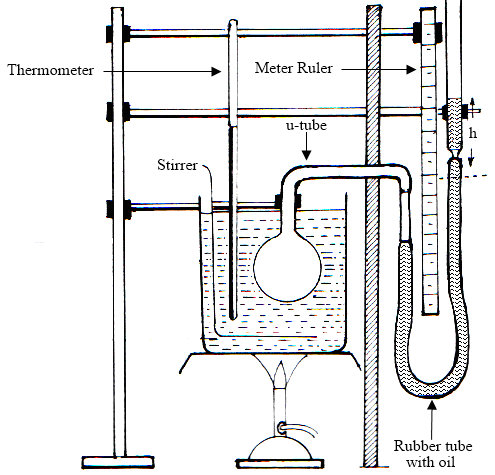
\includegraphics[width=8cm]{./img/pressure-law-1.png}
\caption{Pressure Law practical setup}
\label{fig:pressure-law-1}
\end{figure}

\section{Analysis and Interpretation}
\begin{enumerate}
\item Tabulate your results for the value of temperature $\theta$, $h$ and pressure $P=H +\rho gh$ (where $H$ is atmospheric pressure$ = 10^5$ Nm$^2$, $g = 10$ $^{\text{m}}/_{\text{s}^2}$ and $\rho = 800$ $^{\text{kg}}/_{\text{m}^3}$ is the density of the oil).
\item Plot a graph of pressure $P$ against temperature $\theta$, then find the slope.
\item Draw a best fit line which intersects the horizontal axis.
\item What is the value of $\theta$ when pressure $P$ equals zero?
\end{enumerate}

\section{Conclusion}
What is the relationship between pressure and temperature of a fixed mass of gas at constant volume?

\section{Questions for Discussion}
\begin{enumerate}
\item What does pressure $P$ represent?
\item What is the meaning of the value of $\theta$ obtained when pressure $P$ equals zero?
\item Does the volume of the gas remain constant? If not, how does this affect your results?
\item What cause the pressure to increase when a gas is heated at constant volume?
\end{enumerate}

\section{Reflection and Self Assessment}
\begin{enumerate}
\item What is the application of this experiment in your daily life?
\item Is there anything you do not understand in this experiment? If so, what is it and in what ways can you improve your understanding.
\end{enumerate}